% Copyright (C) 2014 by Thomas Auzinger <thomas.auzinger@cg.tuwien.ac.at>

\documentclass[draft,final]{vutinfth} % Remove option 'final' to obtain debug information.

% Extended LaTeX functionality is enables by including packages with \usepackage{...}.
\usepackage{fixltx2e}  % Provides fixes for several errors in LaTeX2e.
\usepackage{amsmath}   % Extended typesetting of mathematical expression.
\usepackage{amssymb}   % Provides a multitude of mathematical symbols.
\usepackage{mathtools} % Further extensions of mathematical typesetting.
\usepackage{microtype} % Small-scale typographic enhancements.
\usepackage{enumitem}  % User control over the layout of lists (itemize, enumerate, description).
\usepackage{multirow}  % Allows table elements to span several rows.
\usepackage{booktabs}  % Improves the typesettings of tables.
\usepackage[ruled,linesnumbered,algochapter]{algorithm2e} % Enables the writing of pseudo code.
\usepackage{nag}       % Issues warnings when best practices in writing LaTeX documents are violated.
\usepackage{hyperref}  % Enables cross linking in the electronic document version. This package has to be included second to last.
\usepackage[acronym,toc]{glossaries} % Enables the generation of glossaries and lists fo acronyms. This package has to be included last.

\usepackage{tikz}
\usepackage{placeins}

\newcommand{\hl}{\par\medskip\noindent}
\newcommand{\dl}{\par\bigskip\noindent}

\setsecnumdepth{subsection} % enumerate subsections

% Use an optional index
\makeindex
% Use an optional glossary
\makeglossaries
%\glstocfalse % remove the glossaries from the table of contents

% Set persons with 4 arguments:
%  {title before name}{name}{title after name}{gender}
%  where both titles are optional (i.e. can be given as empty brackets {})
\setauthor{}{Patrick Bellositz}{}{male}
\setadvisor{Ao.Prof.Dipl.-Ing.Dr.techn.}{Christian Georg Ferm{\"u}ller}{}{male}

% Required data
\setaddress{Eichkogelstra{\ss}e 10/10/9, 2353 Guntramsdorf}
\setregnumber{1027108}
\setdate{01}{06}{2015}
\settitle{Abstract Argumentation Frameworks}{Abstract Argumentation Frameworks} % sets English and German version of the title (both can be English or German)

\setthesis{bachelor}

% For bachelor and master
\setcurriculum{Software \& Information Engineering}{Software \& Information Engineering} % sets the English and German name of the curriculum

\begin{document}

\frontmatter % switches to roman numbering
% The structure of the thesis has to conform to
%  http://www.informatik.tuwien.ac.at/dekanat

%\addtitlepage{naustrian}
\addtitlepage{english} % English title page
\addstatementpage

\begin{danksagung*}
Ihr Text hier.
\end{danksagung*}

\begin{acknowledgements*}
Enter your text here.
\end{acknowledgements*}

\begin{abstract}
Enter your text here.
\end{abstract}

% Select the language of the thesis, e.g., english or naustrian.
\selectlanguage{english}

% Add a table of contents (toc)
\tableofcontents % starred version, i.e., \tableofcontents*, removes the self-entry

% Switch to arabic numbering and start the enumeration of chapters in the table of content.
\mainmatter

\chapter{Introduction}
Enter your text here.

\chapter{Definitions}

To work with argumentation frameworks, first we must define their properties. This section will lay out the basic structure of argumentation frameworks as well as provide extension types for further analysis.\hl

\noindent
\textbf{Definition 1.} An \emph{argumentation framework} $F$ is a pair $(A,R)$, where $A$ is a set of arguments and $R$ is a set of attack relations.\dl
\textbf{Definition 2.} \emph{Attack relations} $R\subseteq A\times A$ represent attacks. The pair $(a,b)$, where $a,b\in A$ means $a$ \emph{attacks} $b$.\dl
\textbf{Example 1.} Imagine we have 3 arguments $a_1$, $a_2$, and $b$.\hl
			\begin{tabular}{p{0.5cm}p{0.5cm}l}
			& $a_1$ & = ''Blue is the most beautiful of all colors.''\\
			& $b$ & = ''No, black is much more beautiful!''\\
			& $a_2$ & = ''That's wrong, black isn't even a color.''
			\end{tabular}\hl
These arguments obviously contain 2 attacks. Argument $b$ attacks argument $a_1$ and in turn argument $a_2$ attacks argument $b$.\hl
This results in the framework $F=(A,R)$, where $A=\{a_1,a_2,b\}$ and $R=\{(b,a_1),(a_2,b)\}$.\dl
As writing an argument framework in sets might become hard to read with increasing set sizes, it is also possible to write every framework as a graph $(V,E)$, where $V=A$ and $E=R$. The graph in our example looks like this:\dl

\FloatBarrier
	\begin{figure}[!htb]
		\centering
		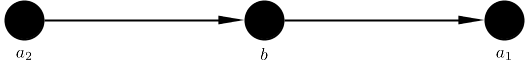
\includegraphics[width=\linewidth]{graphs/ex1.png} %causes underfull hbox and Remark 1 isn't in line with the other txtbf's
		\caption{An argument framework about colors.}
	\end{figure}
\FloatBarrier

\noindent
\textbf{Remark 1.} Let $S$ be a set of arguments. If $a\in S$ and there is an attack $(a,b)\in R$ we say $S$ \emph{attacks} $b$.\dl
\textbf{Definition 3.} Let $S$ be a set of arguments. It is \emph{conflict-free}, if $\forall a \forall b\ a,b\in S, (a,b)\notin R$.\dl
\textbf{Example 2.} (Continuation of Example 1) As no argument attacks itself, $\{a_1\}$, $\{a_2\}$ and $\{b\}$ each are conflict-free. $\{a_1,a_2\}$ is also a conflict-free set, since there exists no attack relation containing $a_1$ and $a_2$. The empty set is always conflict-free.\\
Since there is an attack relation between $b$ and each of the other arguments, there are no other conflict-free sets.\hl
Thus the set of conflict-free sets is $cf(F)=\{\emptyset,\{a_1\},\{a_2\},\{b\},\{a_1,a_2\}\}$.\dl
\textbf{Definition 4.} An argument $a$ is \emph{defended} by a set $S$, if for every attack $(b,a)\in R$ there is an attack $(c,b)$, where $c\in S$. If this is the case $S$ \emph{defends} $a$.\dl
\textbf{Definition 5.} Let $S$ be a conflict-free set. It is called an \emph{admissible extension} if it defends each $a\in S$.\dl
\textbf{Example 3.} (Continuation of Example 2) Of the conflict-free sets only $\{a_2\}$ and \(\emptyset\) don't get attacked. They are admissible. $\{a_1,a_2\}$ gets attacked via the attack relation $(b,a_1)$, but $a_1$ gets defended through $(a_2,b)$, making it also admissible.\\
$\{b\}$ and $\{a_1\}$ are not admissible since they don't defend their arguments.\hl
Thus the set of admissible extensions is $adm(F)=\{\emptyset,\{a_1,a_2\},\{a_2\}\}$.\dl
\textbf{Definition 6.} Let $S$ be an admissible extension. It is called a \emph{preferred extension} if for each $S'\subseteq A$, that is an admissible extension, $S\not\subset S'$.\dl
\textbf{Example 4.} (Continuation of Example 3) Since $\emptyset\subset\{a_2\}$, \(\emptyset\) is not a preferred extension. $\{a_2\}\subset\{a_1,a_2\}$, therefore $\{a_2\}$ is not a preferred extension.\\
Since all other admissible extensions are proper subsets of $\{a_1,a_2\}$, it is a preferred extension.\hl
Thus the set of preferred extensions is $prf(F)=\{\{a_1,a_2\}\}$.\dl
\textbf{Definition 7.} Let $S$ be a conflict-free set. It is called a \emph{stable extension} if for each $a\not\in S$ there is exists an attack $(b,a)\in R$ where $b\in S$.\dl
\textbf{Example 5.} (Continuation of Example 2) The conflict-free sets $\emptyset$ and $\{a_1\}$ don't attack any of the other arguments, $\{a_2\}$ only attacks $\{b\}$, missing an attack on $\{a_1\}$. $\{b\}$ misses an attack on $\{a_2\}$. They are not stable extensions.\\
$\{a_1,a_2\}$ attacks all other arguments in $\{b\}$ (attack relation $(a_2,b)$) and therefore is a stable extension.\hl
Thus the set of stable extensions is $st(F)=\{\{a_1,a_2\}\}$.\dl
\textbf{Definition 8.} Let $S$ be an admissible extension. It is called a \emph{complete extension} if for each $a\not\in S$, $S\cup \{a\}$ is not an admissible extension.\dl
\textbf{Example 6.} (Continuation of Example 3) The admissible extension $\emptyset$ is not a complete extension because it defends $a_2$ which it doesn't contain. $\{a_2\}$ defends $a_1$ and is therefore also not a complete extension.\\
$\{a_1,a_2\}$ attacks $b$ and as there are no other arguments which could be defended it is a complete extension.\hl
Thus the set of complete extensions is $co(F)=\{\{a_1,a_2\}\}$.\dl
\textbf{Definition 9.} The (unique) \emph{grounded extension} is defined by $\bigcap\limits_{i=1}^n{S_i}$, where $\{S_1,...,S_n\}$ is the set of all complete extensions.\dl
\textbf{Example 7.} (Continuation of Example 6) Since there is only one complete extension $\{a_1,a_2\}$, it also is the grounded extension $gr(F)$.\dl

\chapter{Observations}

As we have seen in the previous section%change sentence if it is not the previous one anymore
, often there may be overlaps between the different extension types beyond what their definitions explicitly state. In this section we will discuss those relations between extension types.\dl

\FloatBarrier
	\begin{figure}[!htb]
		\centering
		\begin{tikzpicture}[fill=white]
			\scope
				\clip (-2,-2) rectangle (2,2)
					(1,0) circle (1);
				\fill (0,0) circle (1);
			\endscope
			\scope
				\clip (-2,-2) rectangle (2,2)
					(0,0) circle (1);
				\fill (1,0) circle (1);
			\endscope
			\draw (3.5,3.5) circle (4.75) (3.5,7.75) node [text=black,above] {cf}
				(3.5,3.5) circle (4) (3.5,7) node [text=black,above] {adm}
				(2.25,4.25) circle (1.75) node [text=black] {prf}	
				(4.75,4.25) circle (1.75) node [text=black] {st}
				(3.5,2) circle (1.75) (3.5, 1.5) node [text=black] {co}
				(3.5,2.75) circle (.75) (3.5, 2.5) node [text=black] {gr}
				(-2,-2) rectangle (9,9) (3.5,8.75) node [text=black]{all sets};
		\end{tikzpicture}
		\caption{Relations between extension types}
	\end{figure}
\FloatBarrier

\chapter{Application}

\section{Introduction}
In this section the usage and implementation details of the aforementioned program illustrating the computation of the different extension types is provided.

\section{Creation of a framework}
On starting the application the user is presented with an input mask. It consists of ten rows, each representing an argument and a button labeled "show graph".

\FloatBarrier
	\centering
	\begin{figure}[!htb]
		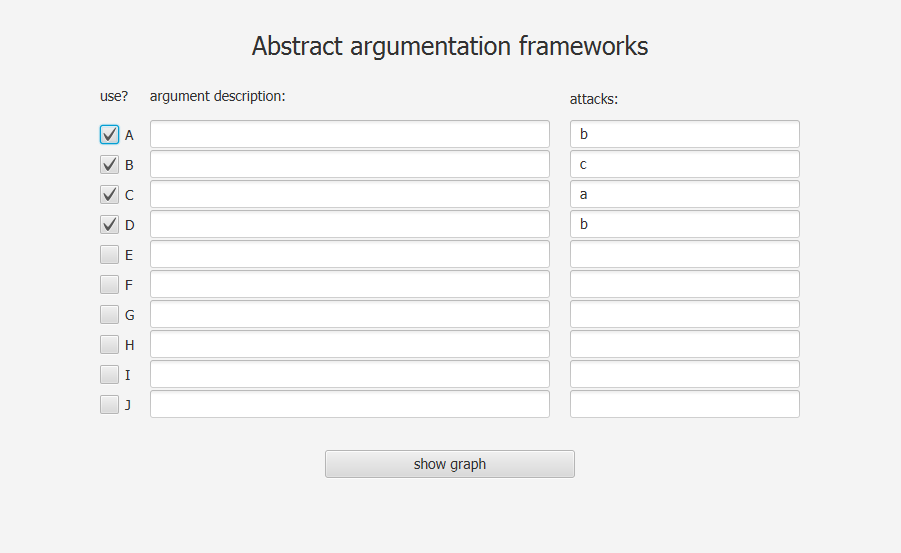
\includegraphics[width=\linewidth]{pics/input.png}
		\caption{Input mask}
	\end{figure}
\FloatBarrier

\section{Argumentation graph}
Once a framework is created and "show graph" was clicked a graphical representation of it is shown alongside buttons to compute extensions and an area dedicated to showing computation results.

\FloatBarrier
	\centering
	\begin{figure}[!htb]
		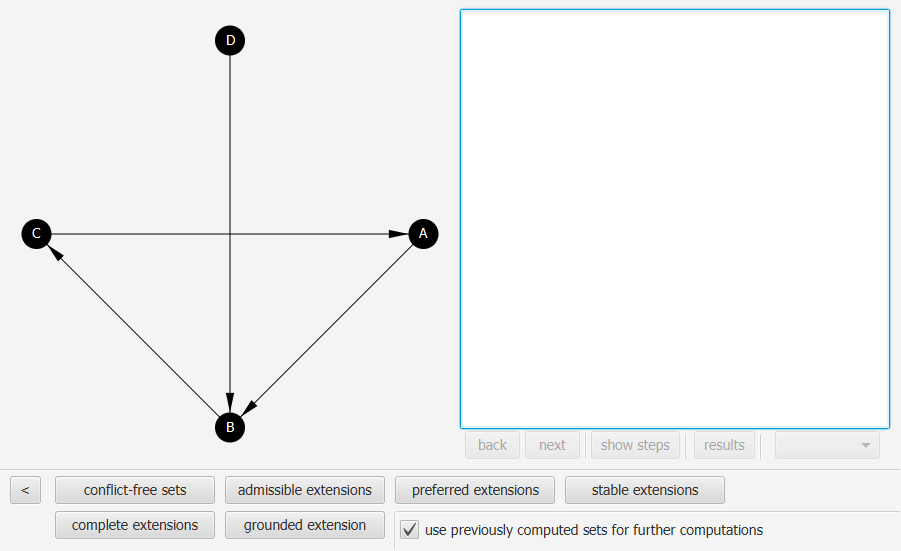
\includegraphics[width=\linewidth]{pics/demo.png}
		\caption{Demonstration view}
	\end{figure}
\FloatBarrier

\section{stuff comes here}

\backmatter

% Add a bibliography
\bibliographystyle{alpha}
\bibliography{intro}

% Add an index
\printindex

% Add a glossary
\printglossaries

\end{document}